\chapter{Бинарные оптимизации на основе трасс исполнения}\label{ch:ch4}

В этой главе приведено описание бинарных оптимизаций на основе трасс исполнения приложения.

В разделе 4.1 описываются проблемы оптимизаций с профильной информацией. Приводится пример приложения, когда от выбранного сценария зависит, будет получен прирост, или регрессия производительности на приложении.

В разделе 4.2 рассматривается дополнительная информация, которую возможно извлечь из трассы исполнения и применить для последующей бинарной оптимизации приложения.

В разделе 4.3 приводится описание мультипрофильного анализа трасс исполнения приложения. Вводятся основные необходимые термины для данного анализа: интервалы инструкций, фазы исполнения и мультипрофиль.

В разделе 4.4 описывается бинарная оптимизация - дублирование кода на основе мультипрофиля. Рассматриваются основные случаи применимости данной оптимизации.

В разделе 4.5 приводятся результаты запусков тестов, оптимизированных с помощью дублирования кода на основе мультипрофиля.

\section{Проблемы оптимизации с профильной информацией}\label{sec:ch4/sect1}
Профилирование программы – это сбор характеристик работы программы. При работе оптимизатора BOLT необходимы значения счетчика команд и последние взятые переходы с информацией от предсказателя переходов. Во время сбора характеристик программа исполняется по определенному сценарию: конкретные входные данные, параметры окружения, контекст и т.д. Полученная профильная информация будет показывать характеристики этого выбранного сценария.

После оптимизации приложения с данным профилем запуск по данному сценарию будет показывать прирост производительности, но при проверке производительности с другими входными параметрами на данном приложении такого же прироста производительности получить не удастся (вероятно будет происходить регрессия) \cite{Valiante2021}.

Рассмотрим демонстрационное приложение (рисунок \cref{fig:TestCode}), которое может иметь два сценария исполнения.

После сбора профилировочной информации и прохождений оптимизаций BOLT расположит часто использованные линейные участки в секции кода .text, остальные будут размещены в секции кода .text.cold (рисунок \cref{fig:CFGProfile1}).
 
\begin{figure}[!h]
    \centerfloat{
        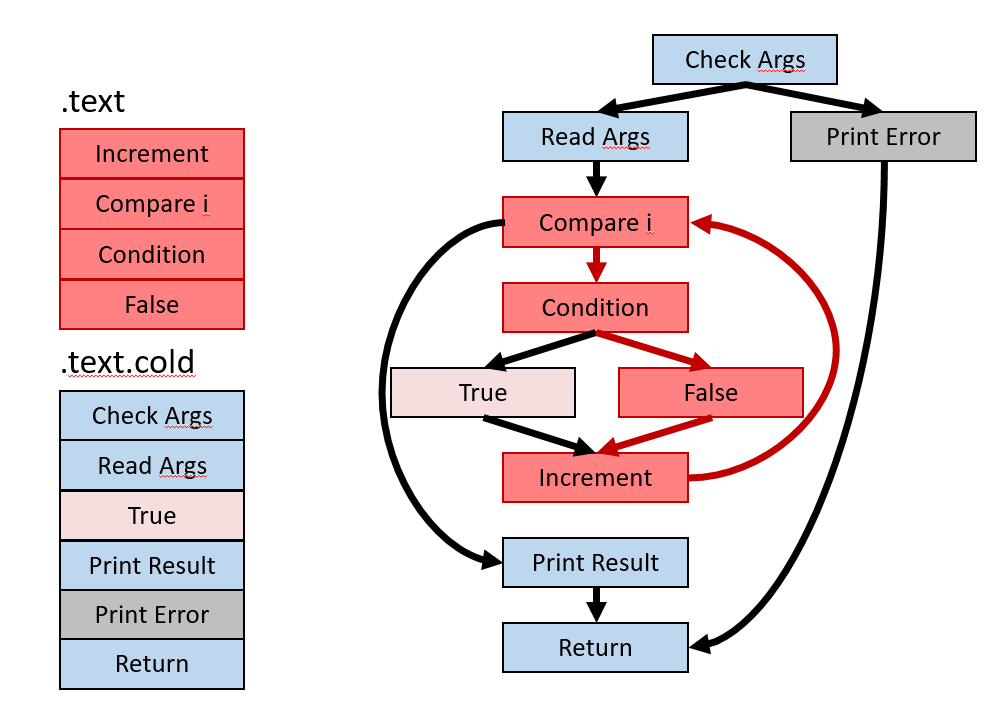
\includegraphics[width=0.8\linewidth]{_3}
    }
    \caption{Граф потока управления с профилем}\label{fig:CFGProfile1}
\end{figure}
Для собранного профиля приложение стало более производительным за счёт расположения всего горячего кода в одном месте. Однако, если исполнение пойдет по другому пути, то производительность понизится из-за перехода в горячий линейный участок «True», расположенный в другой секции (рисунок \cref{fig:CFGProfile2}).

\begin{figure}[!h]
    \centerfloat{
        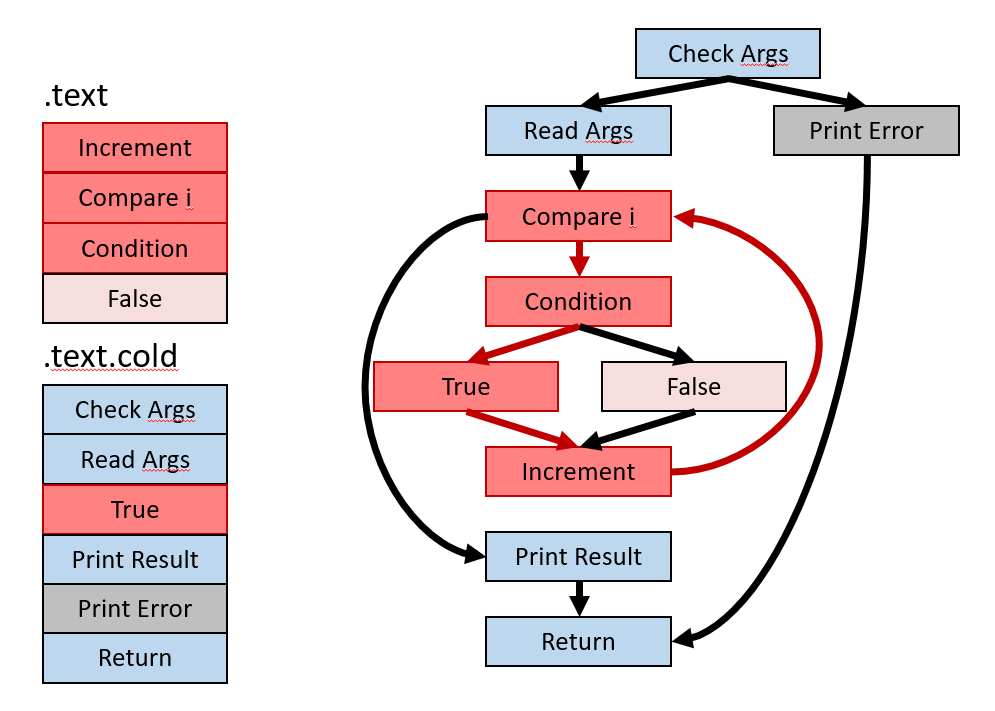
\includegraphics[width=0.8\linewidth]{_4}
    }
    \caption{Граф потока управления с измененным профилем}\label{fig:CFGProfile2}
\end{figure}

Для решения данной проблемы необходимо покрыть все возможные сценарии работы данного приложения. В итоге получив запуски с горячими линейными участками как «True», так и «False», суммарная профильная информация позволит BOLT расположить обе ветки исполнения в оптимизированной секции вместе (рисунок \cref{fig:CFGProfile3})\cite{Lin2021}.
 
\begin{figure}[!h]
    \centerfloat{
        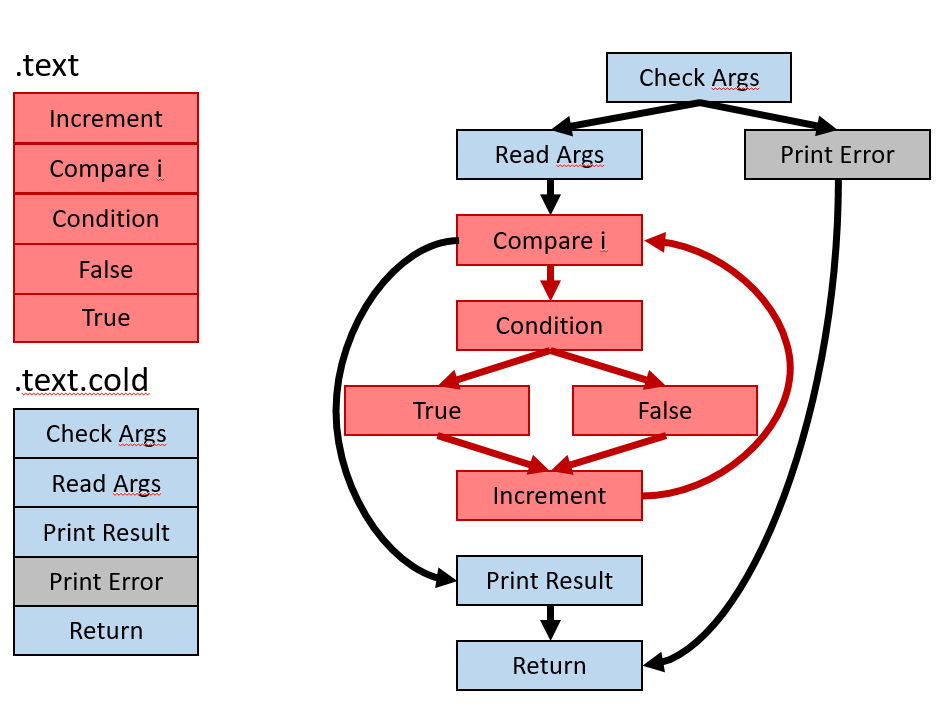
\includegraphics[width=0.8\linewidth]{_5}
    }
    \caption{Граф потока управления с суммарным профилем}\label{fig:CFGProfile3}
\end{figure}
Теперь выделенными в горячую секцию оказываются два сценария. Если при запуске используется только один сценарий, то второй будет занимать место в оптимизированной секции. Учитывая расположение в новой секции линейных участков, предпочтительнее использовать «False» ветку, так как она лежит непосредственно после участка «Condition». В случае с веткой «True» будет происходить захват линейного участка «False».

Для того чтобы этого не происходило, необходимо произвести копирование горячих линейных участков, которые относятся к различным сценариям: линейные участки «Increment» «Compare i» «Condition». Таким образом, будут созданы их копии сценария «True»: «Increment*» «Compare i*» «Condition*» (рисунок \cref{fig:CFGProfile4}).
 
\begin{figure}[!h]
    \centerfloat{
        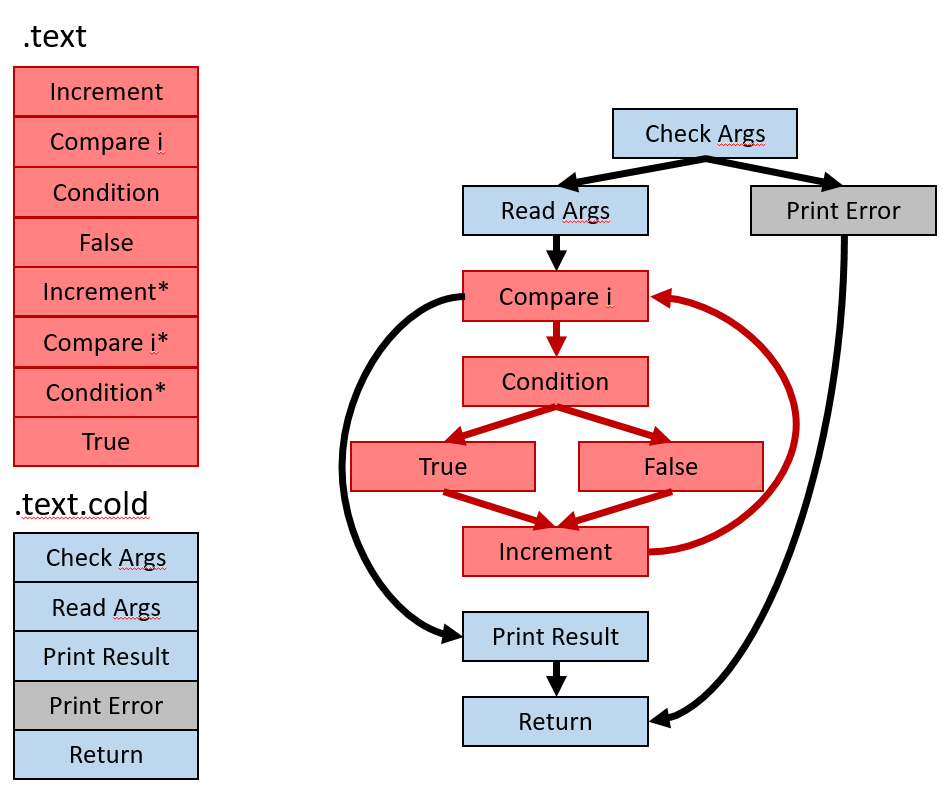
\includegraphics[width=0.8\linewidth]{_6}
    }
    \caption{Оптимизированная секция с дублированием кода}\label{fig:CFGProfile4}
\end{figure}
После всех преобразований полученная оптимизированная секция будет содержать в себе два непересекающихся сценария.

Рассмотрим, как будет происходить выбор исполняемого сценария (рисунок \cref{fig:CFGSec1}). После запуска приложения, проверки и считывания аргументов исполнение переходит в линейный участок «Compare i» произвольного сценария (для определенности «False»). После этого в линейном участке «Condition» будет происходить выбор нужной ветки исполнения. Это приведет к выбору сценария, по которому пойдёт дальнейшее исполнение.

 
\begin{figure}[!h]
    \centerfloat{
        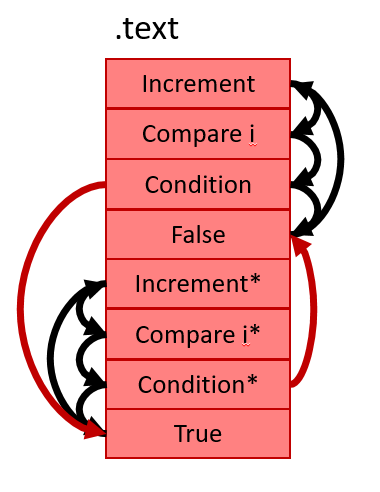
\includegraphics[width=0.5\linewidth]{_7}
    }
    \caption{Поток управления по секции с дублированием кода}\label{fig:CFGSec1}
\end{figure}
На рисунке красными стрелками отображены переходы между сценариями. Из-за дублирования кода размер секции стал больше, но таким образом удалось изолировать сценарии друг от друга. Однако, если будут частые переключения между ними, то в итоге количество постоянно исполняемого кода будет включать себя и оригинальные линейные участки, и их дубликаты. Самый сложный случай – чередование сценариев «True» и «False». В этом случае последовательность исполнения будет следующая:
«Condition» => «True» => «Increment*» => «Compare i*» => «Condition*» => «False» => «Increment» => «Compare i» => «Condition» => «True» => …
В итоге получается 4 варианта реализации оптимизированной секции (рисунок \cref{fig:CFGSec2}).
 
\begin{figure}[!h]
    \centerfloat{
        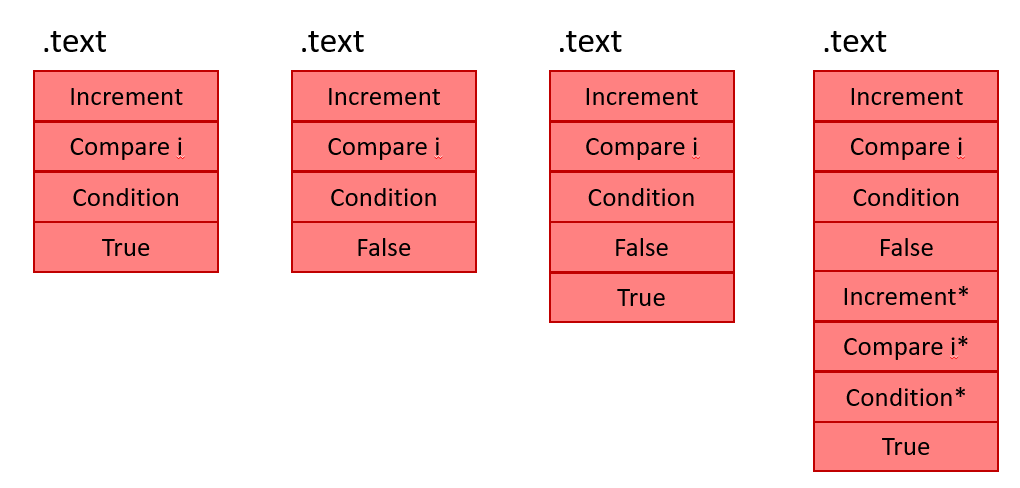
\includegraphics[width=1.0\linewidth]{_8}
    }
    \caption{Варианты оптимизированных секций}\label{fig:CFGSec2}
\end{figure}
Первые два варианта подходят только в том случае, если есть уверенность в отсутствии запусков сценариев, не помещенных в секцию. При наличии исполнения обоих сценариев и частом переключении между ними необходимо использовать третий вариант секции. И если переключения между сценариями редкие, то необходимо использовать 4 вариант, вариант оптимизированной секции с дублированием общего кода.
На практике можно реализовать несколько случаев в бинарном файле и поставить специальные счетчики, которые будут перенаправлять между вариантами оптимизированных секций, но данный вариант рассматриваться не будет.

Приведенный пример содержит в себе мало исполняемого кода, поэтому дублирование кода не сильно увеличит размер секции, но если рассмотреть примеры реальных приложений, пересечение между сценариями могут покрывать больше половины секции кода. В данном варианте анализ сценариев исполнения и доказательство необходимости дублирования кода становится важной задачей для повышения производительности приложения.

Трасса исполнения содержит в себе гораздо больше информации, чем профиль, который в конечном итоге используется для оптимизации приложения. Помимо количества сделанных переходов на каждой инструкции изменения программного счетчика есть информация о последовательности сделанных переходов, которую можно учитывать во время оптимизации.

Также для оптимизации можно добавить в трассу информацию про использованные адреса в инструкциях загрузки и выгрузки. Таким образом, можно достать подробную информацию для оптимизации данных в бинарном файле.

\section{Мультипрофильный анализ трасс исполнения}\label{sec:ch4/sect3}
Для проведения анализа приложения необходимы трассы исполнения, собранные с помощью динамической бинарной инструментации\cite{Rimsa2021} и покрывающие большинство сценариев использования приложения \cite{confbib3}. В итоге необходимо получить соотношение кода с выявленными сценариями. Для операций с первой величиной будет использоваться понятие линейного участка кода (базовый блок). Для действий, связанных со сценариями, будет использоваться понятие фазы из статьи \cite{Vandeputte2007}. В итоге в ходе анализа многопрофильности необходимо построить соответствие между линейными участками и выявленными фазами \cite{Lin2016}.

Трасса разбивается на одинаковые интервалы по количеству инструкций. Это необходимо для анализа исполнения в рамках одного отрезка времени – интервала инструкций, так как требуется найти похожие интервалы и объединить их в фазы \cite{Lebras2019}.

Для большей наглядности граф исполнения отображается в виде тепловой карты. По оси X – интервалы инструкций согласно времени исполнения, по оси Y – номер линейного участка кода (рисунок \cref{fig:HeatMap1}).

\begin{figure}[!h]
    \centerfloat{
        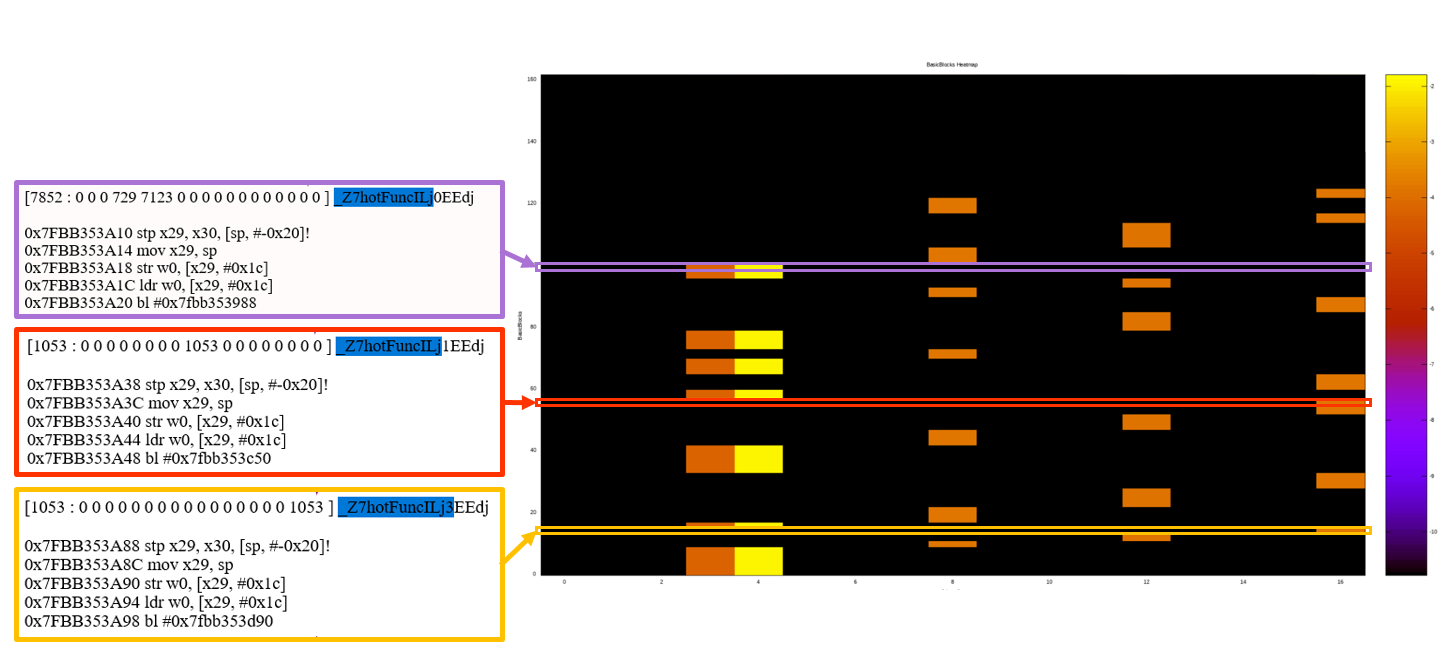
\includegraphics[width=1.0\linewidth]{_9}
    }
    \caption{Построение тепловой карты линейных участков}\label{fig:HeatMap1}
\end{figure}

На каждом интервале исполняется определенный набор линейных участков кода, который характеризует интервал инструкций. Если составить n-мерное пространство, где n – количество линейных участков кода, а координаты – количество исполненных соответствующих линейных участков на выбранном интервале, то каждому интервалу в данном пространстве будет соответствовать точка.

Необходимо произвести кластеризацию интервалов: каждый полученный кластер интервалов инструкций будет означать определенную фазу. Кластеризация будет проводиться с помощью итеративного алгоритма объединения фаз \cite{Vandeputte2007}.

В начале алгоритма каждый интервал считается отдельной фазой. Вычисляются расстояния между текущими фазами, выбирается наименьшее из полученных, и выбранная пара ближайших фаз объединяются. После чего итерация повторяется до тех пор, пока не останется необходимое количество фаз (рисунок \cref{fig:HeatMap2}). Данный алгоритм является жадной кластеризацией, параллельная версия которой была реализована в рамках проделанного исследования.
 
\begin{figure}[!h]
    \centerfloat{
        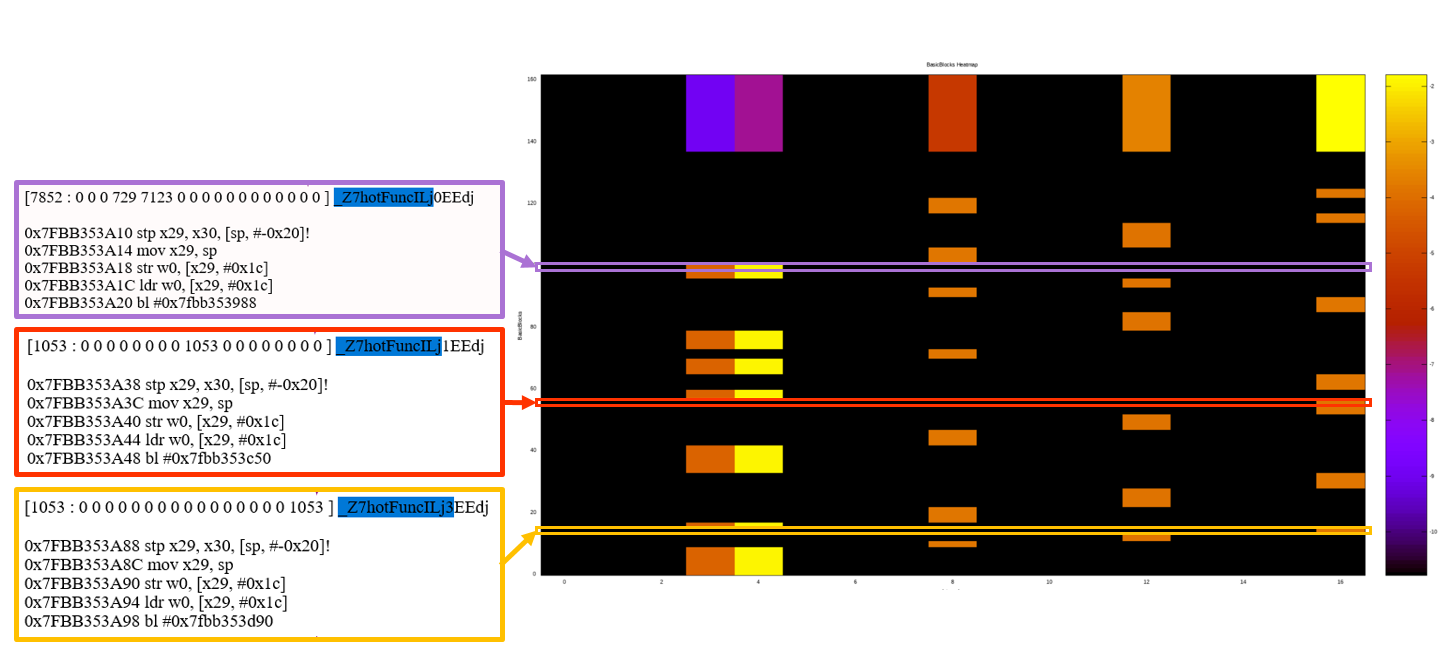
\includegraphics[width=1.0\linewidth]{_10}
    }
    \caption{Добавление фаз исполнения в тепловую карту (верхняя строка тепловой карты)}\label{fig:HeatMap2}
\end{figure}

После выделения фаз начинается стадия их анализа. Для примера анализа рассмотрим приложение с тремя режимами исполнения и без пересечения кода (рисунок \cref{fig:HeatmapEx}).

 
\begin{figure}[!h]
    \centerfloat{
        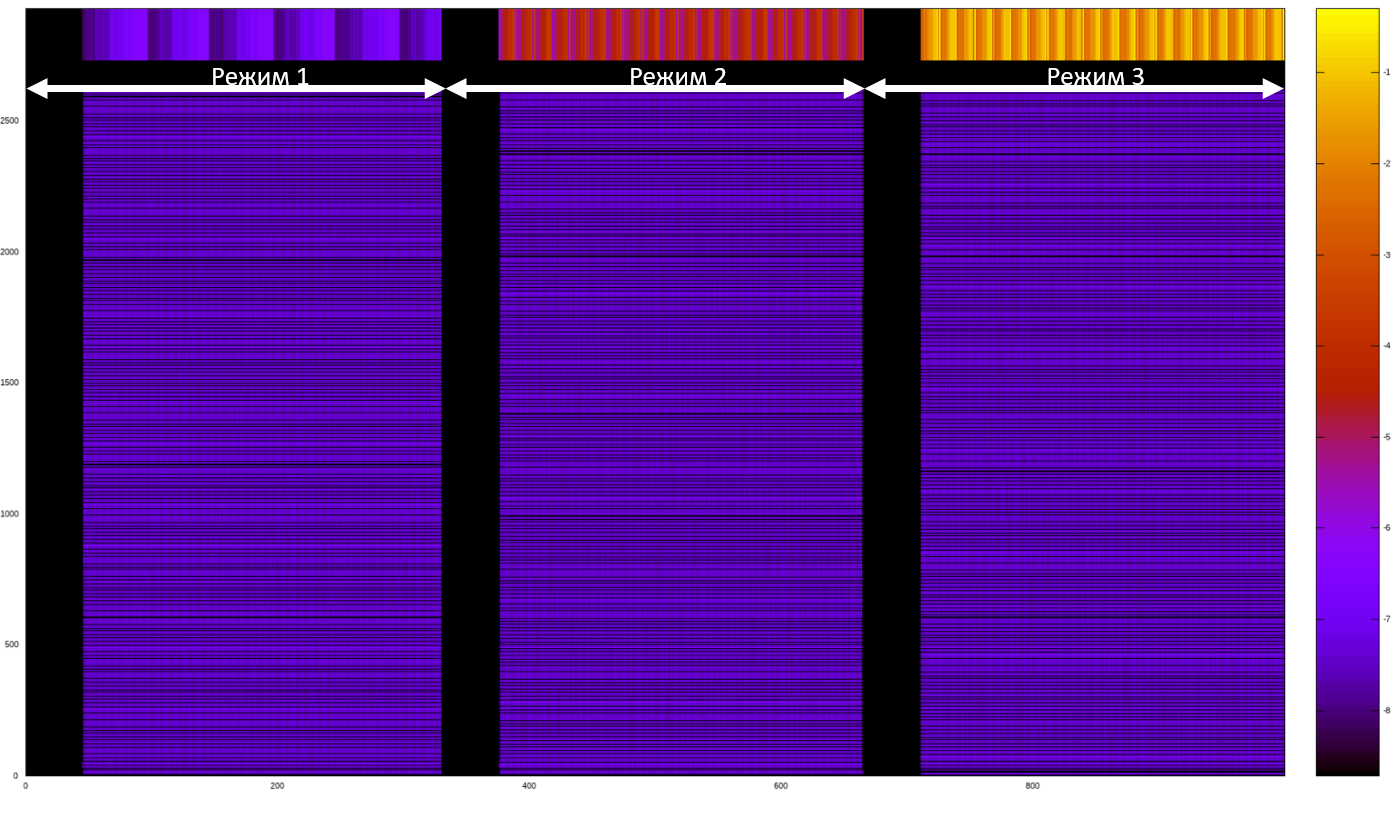
\includegraphics[width=1.0\linewidth]{_11}
    }
    \caption{Тепловая карта приложения, запущенного в трех разных режимах}\label{fig:HeatmapEx}
\end{figure}
По переключениям между фазами строится граф исполнения (рисунок \cref{fig:Phase1}). Он является аналогом графа потока управления, но на более высоком уровне, показывая переключения не между линейными участками, а между макросостояниями исполнения программы.
 

\begin{figure}[!h]
    \centerfloat{
        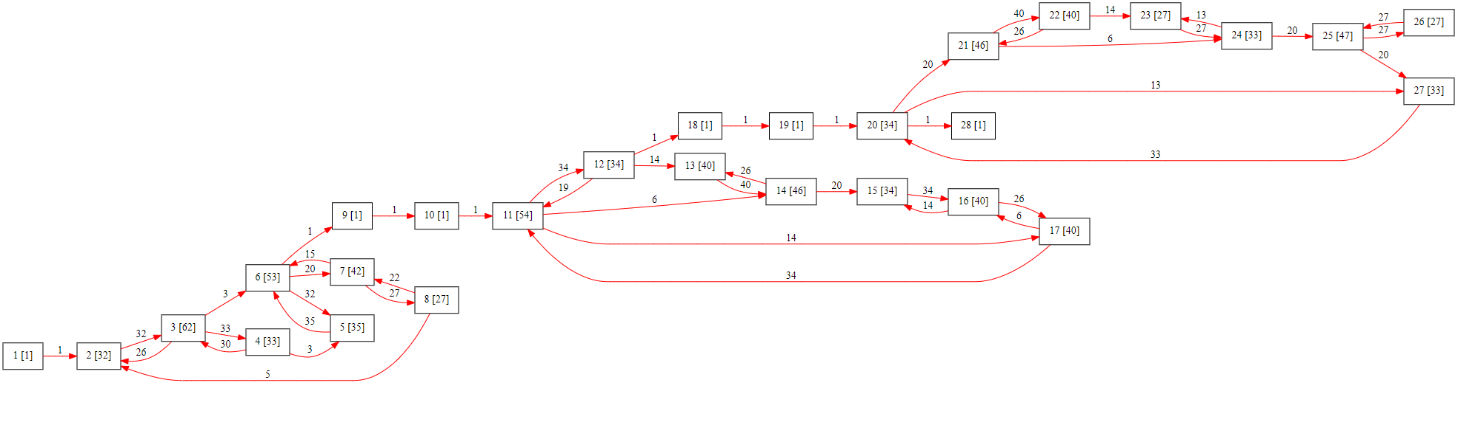
\includegraphics[width=1.0\linewidth]{_12}
    }
    \caption{Граф потока управления по фазам}\label{fig:Phase1}
\end{figure}
Получив граф фаз состояний можно проанализировать сценарии приложения и выделить характерные особенности, используемые затем в оптимизациях.

Если произвести сравнение фаз со сценариями исполнения приложения, то заметна корреляция: на каждый запуск приходятся свои собственные фазы без пересечения (рисунок \cref{fig:Phase2}).
 
\begin{figure}[!h]
    \centerfloat{
        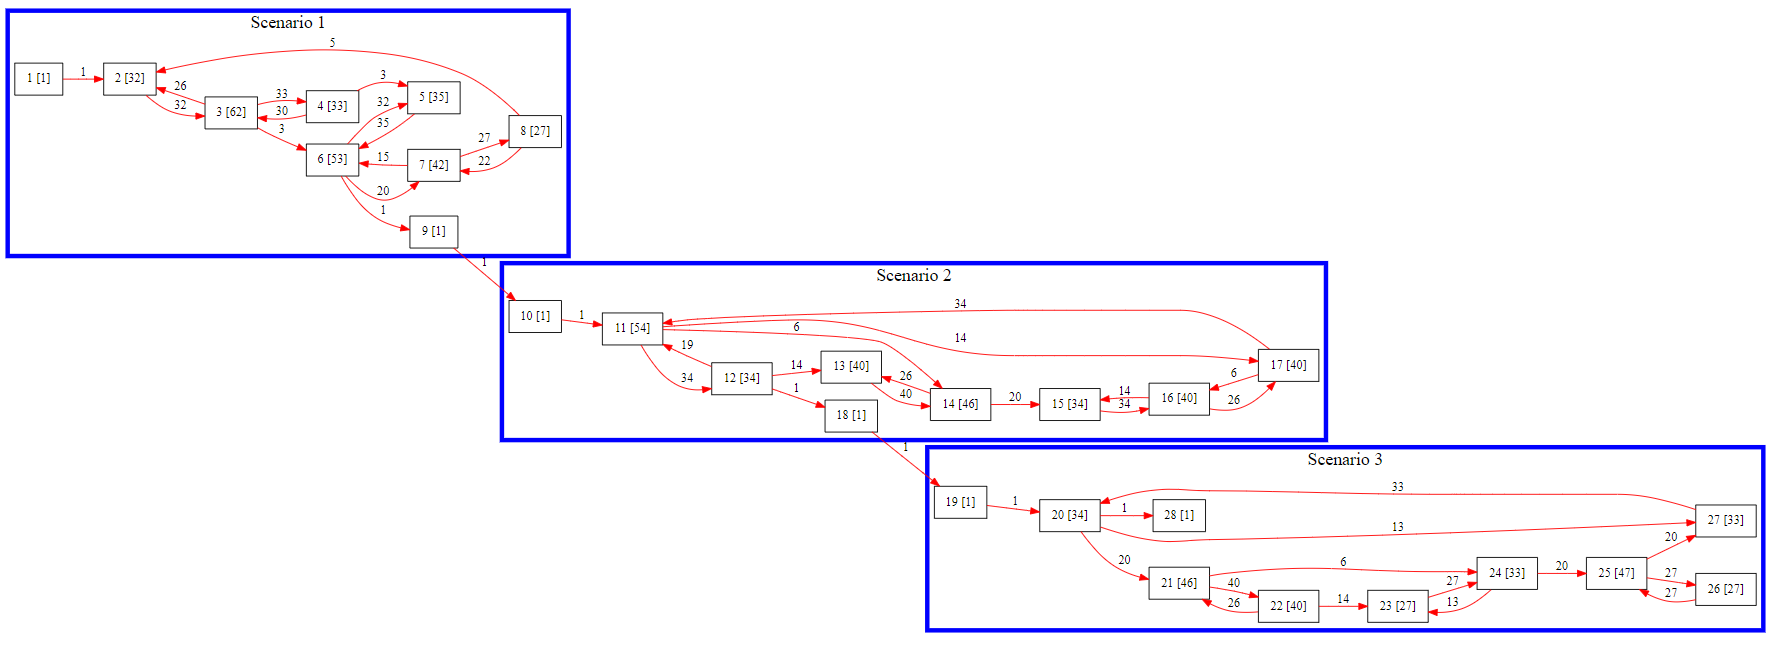
\includegraphics[width=1.0\linewidth]{_13}
    }
    \caption{Соответствие графа потока управления по фазам со сценариями}\label{fig:Phase2}
\end{figure}
Однако, это синтетический пример, поэтому пересечения между сценариями исключены, что позволяет провести оптимизацию перекомпоновки кода без применения дублирования. В реальных приложениях пересечения могут встречаться, и для повышения локальности кода его части необходимо будет дублировать.

Завершение анализа приложения требует построения соответствия между фазами и линейными участками приложения. Для этого каждый линейный участок анализируется отдельно, выбирается интервал с его наибольшим количеством исполнений. Линейному участку кода будет соответствовать фаза, которая включает в себя этот интервал.

В итоге каждому линейному участку кода соответствует фаза, обозначенная на тепловой карте в столбце слева (рисунок \cref{fig:MP1}).
 
\begin{figure}[!h]
    \centerfloat{
        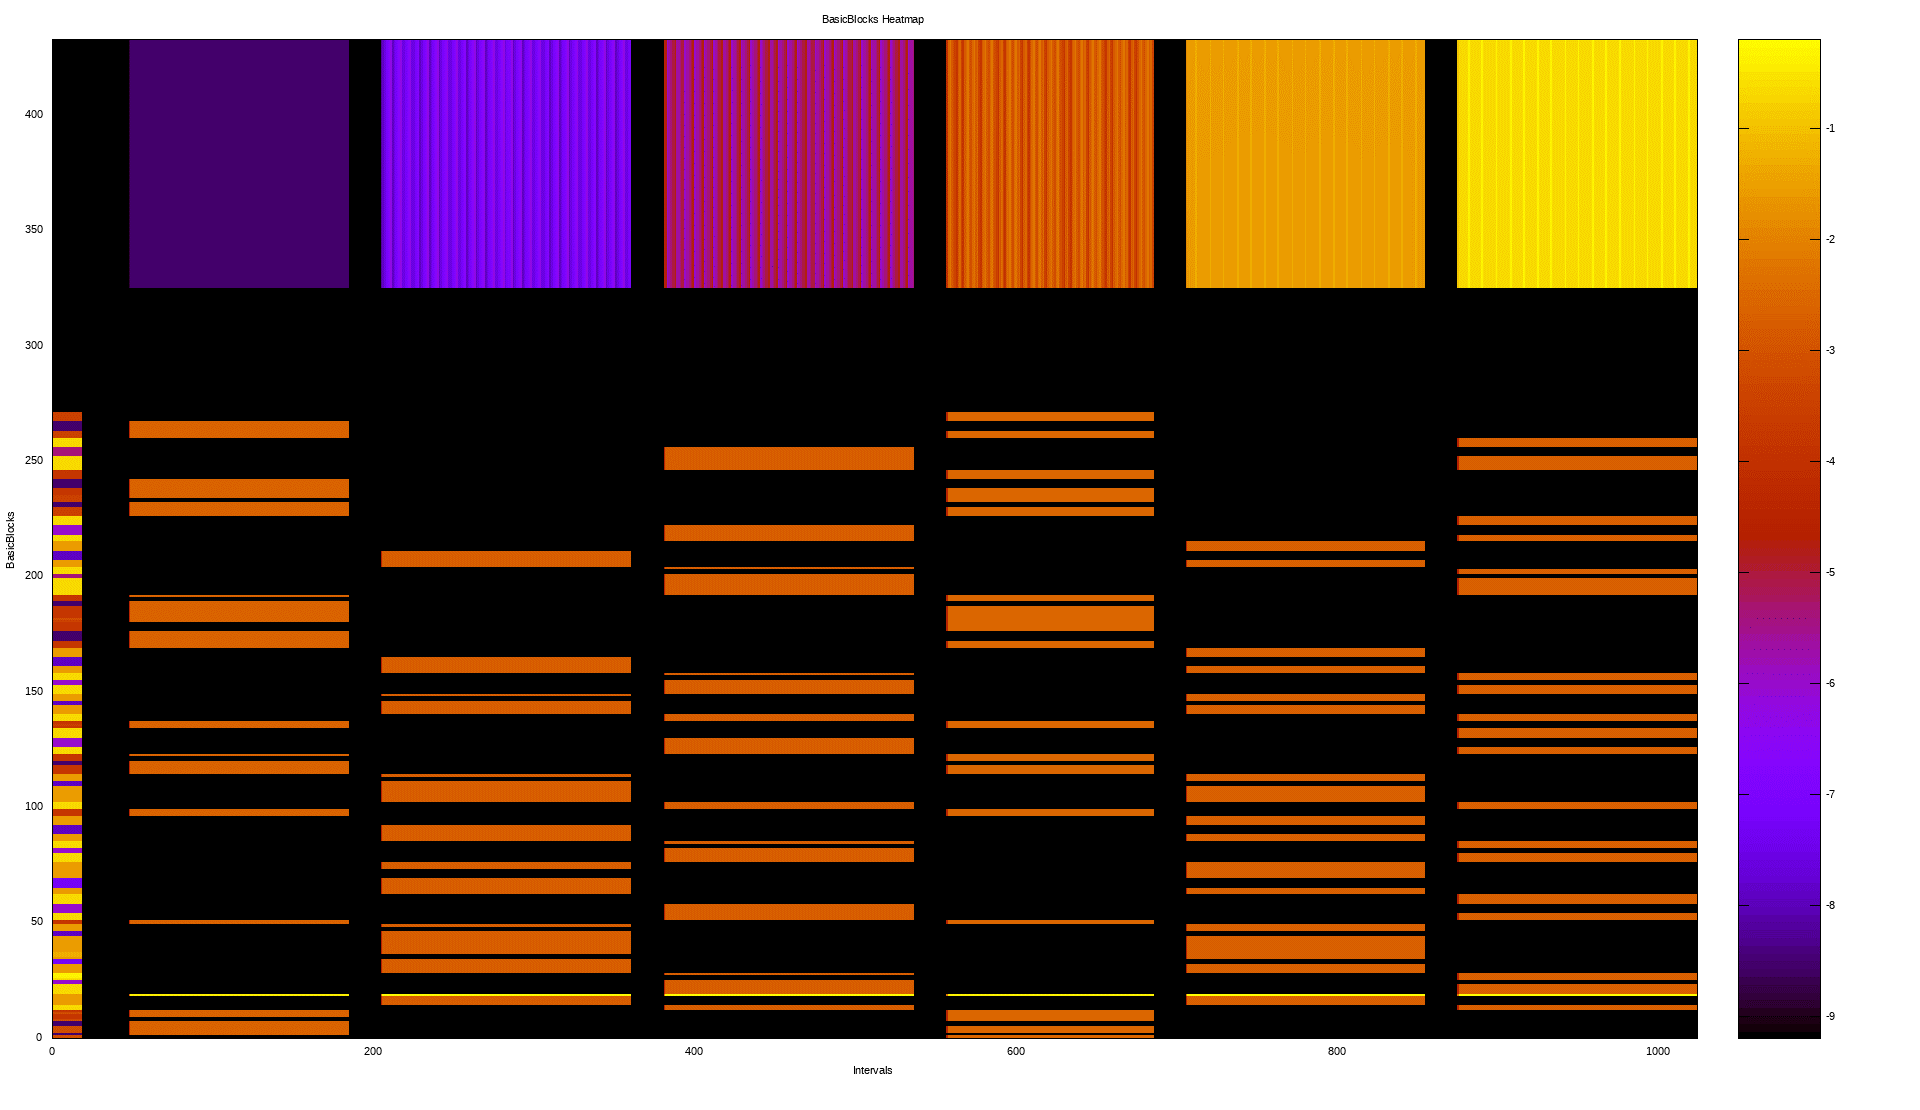
\includegraphics[width=1.0\linewidth]{_14}
    }
    \caption{Пример построения соответствия линейных участков фазам}\label{fig:MP1}
\end{figure}

Получив соответствие линейных участков кода и фаз (рисунок \cref{fig:MP2}), расположение в оптимизированной секции кода будет производиться при размещении всего кода в одной фазе. Для этого производится модификация профильной информации для бинарного оптимизатора BOLT, с прибавлением константы смещения между фазами. Таким образом бинарные функции одной фазы вероятнее окажутся на соседних адресах в оптимизированном бинарном файле (рисунок \cref{fig:MP3}).

Если рассмотреть синтетический тест с разделенными сценариями использованию, то после анализа и оптимизации код будет расположен в оптимизированной секции таким образом, что регионы исполнения сценариев не будут пересекаться.

\begin{figure}[!h]
    \centerfloat{
        \includegraphics[width=1.0\linewidth]{_15а}
    }
    \caption{Пример тепловой карты приложения до сортировки}\label{fig:MP2}
\end{figure}

\begin{figure}[!h]
    \centerfloat{
        \includegraphics[width=1.0\linewidth]{_15б}
    }
    \caption{Пример тепловой карты приложения после сортировки}\label{fig:MP3}
\end{figure}

Без проведения мультипрофильного анализа бинарный оптимизатор BOLT имеет профильную информацию, по которой можно получить подобный результат. На более сложных примерах восстановление глобального потока управления становится неподъемной для BOLTа задачей.

При использовании данного анализа на реальном приложении визуально видно различия в режимах исполнения (рисунок \cref{fig:MP4}). Данные различия позволяют провести отдельный класс приложений, основанный на пересечениях фаз.

\begin{figure}[!h]
    \centerfloat{
        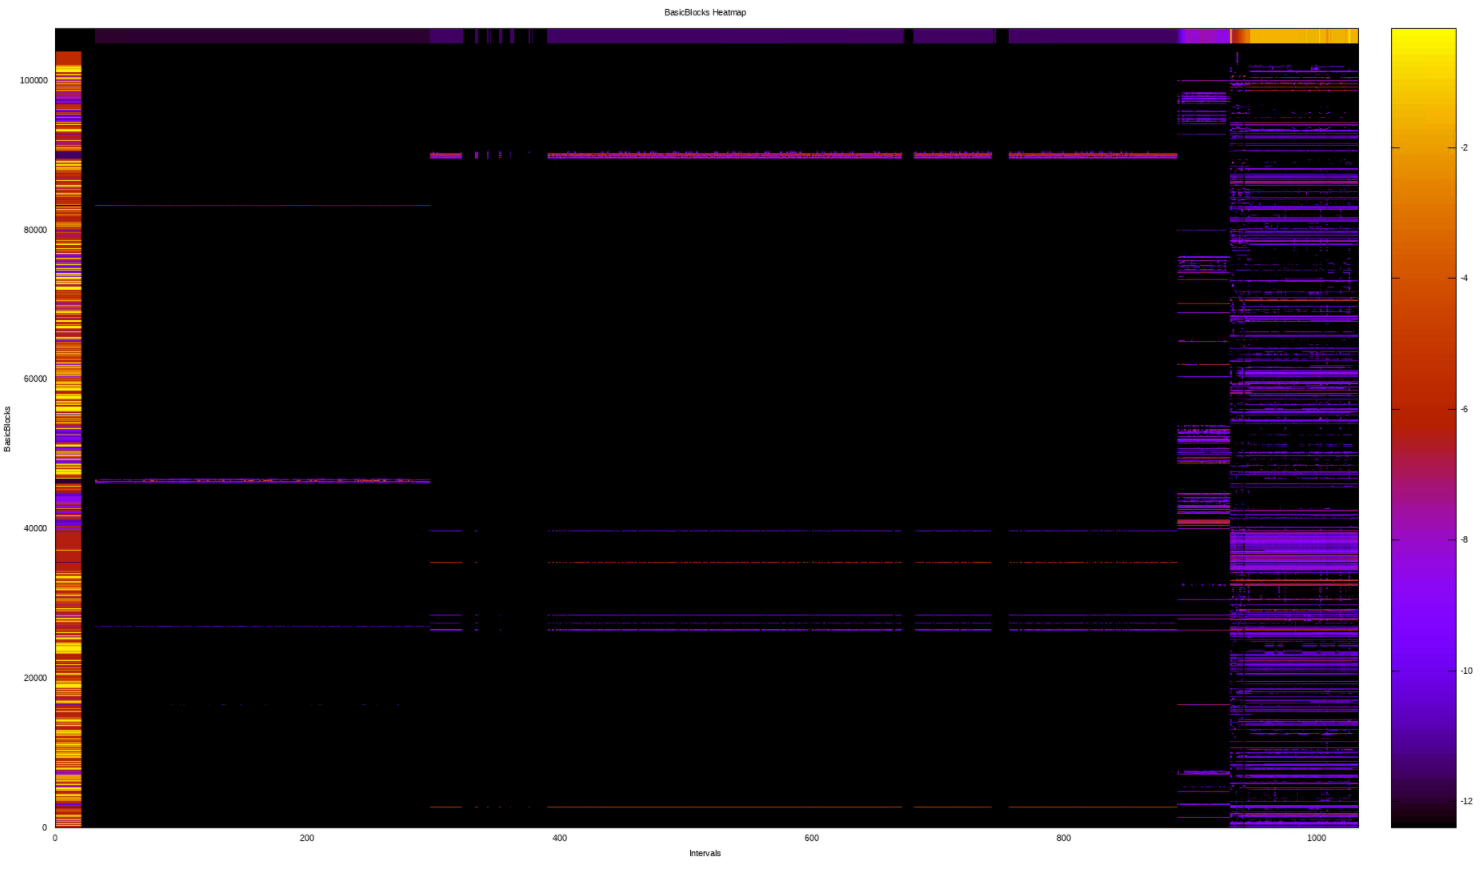
\includegraphics[width=1.0\linewidth]{fortnite}
    }
    \caption{Пример тепловой карты для реальной библиотеки приложения}\label{fig:MP4}
\end{figure}

\section{Дублирование кода на основе мультипрофиля}\label{sec:ch4/sect3}
Выстраивая соответствие между линейными участками кода и фазами, выбиралась фаза, которой принадлежит интервал инструкций с наибольшим количеством исполнений данного линейного участка. Однако, может сложиться ситуация, когда линейный участок одинаково часто исполнялся на интервалах инструкций из разных фаз. В этом случае необходимо запоминать такие линейные участки для последующего анализа необходимости дублирования данного кода \cite{Desmond2009}.

Используя эвристически подобранные соотношения, выбираются те линейные участки, которые относятся одновременно к нескольким фазам. После этого данные участки помечаются для дублирования бинарным оптимизатором BOLT (рисунок \cref{fig:MPOpt}).

\begin{figure}[!h]
    \begin{minipage}[b][][b]{0.49\linewidth}\centering
        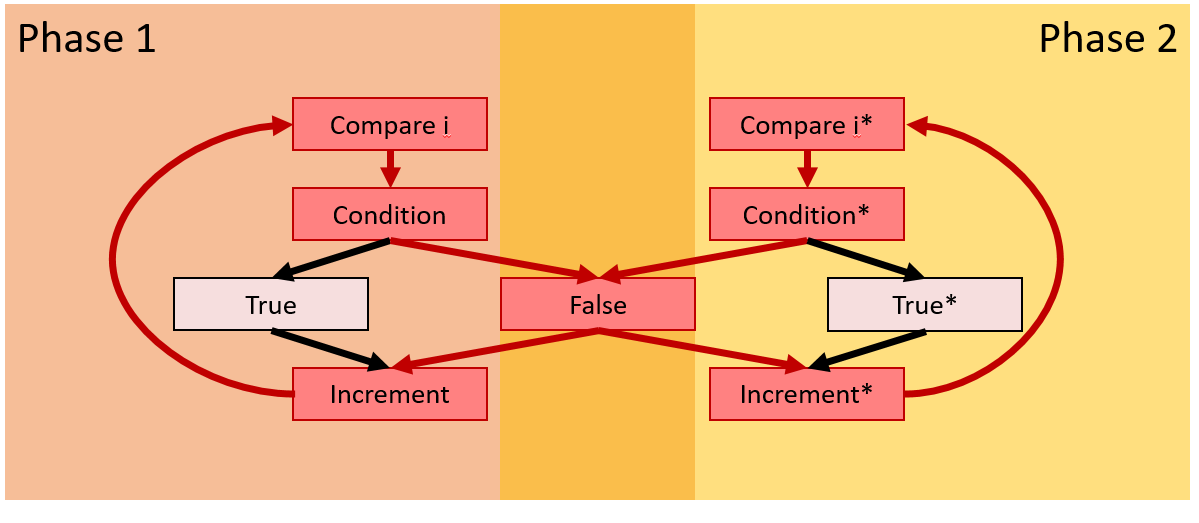
\includegraphics[width=1.0\linewidth]{mi1} \\ а)до оптимизации
    \end{minipage}
    \hfill
    \begin{minipage}[b][][b]{0.49\linewidth}\centering
        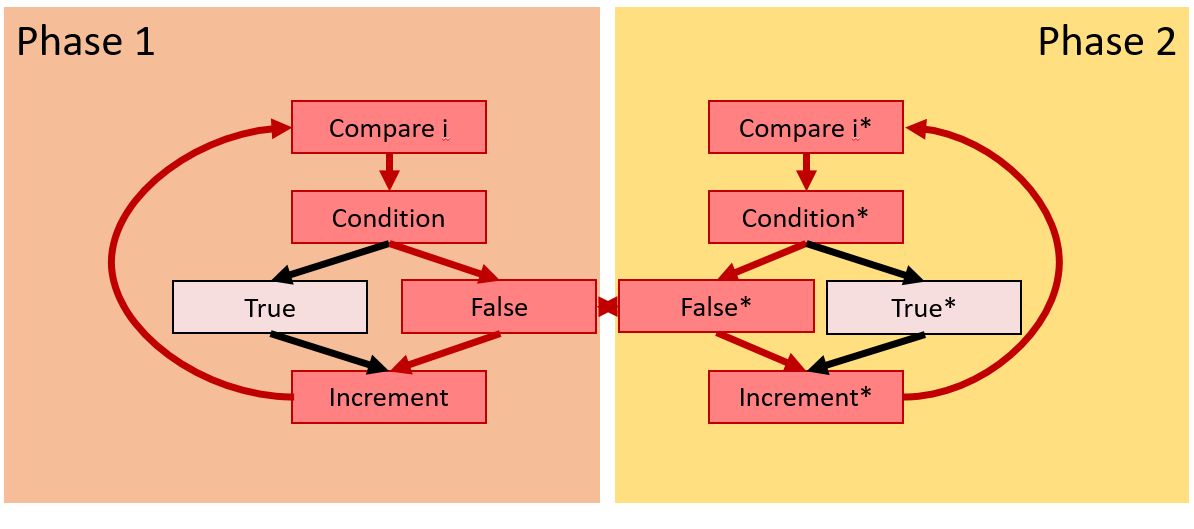
\includegraphics[width=1.0\linewidth]{mi2} \\ б)после оптимизации
    \end{minipage}
    \caption{Дублирование кода на основе мультипрофиля}
    \label{fig:MPOpt}
\end{figure}

\section{Результаты тестирования оптимизации дублирования}\label{sec:ch4/sect3}
Для проверки анализа был использован набор тестов GeekBench (рисунок \cref{fig:GKBMP}). Были записаны трассы его исполнения на различных задачах. На тепловой карте выделены запуски различных задач, представляющие в данном случае сценарии запуска приложения. По верхней строке тепловой карты видно корректное выделение фаз на каждый отдельный тест из набора.

\begin{figure}[!h]
    \centerfloat{
        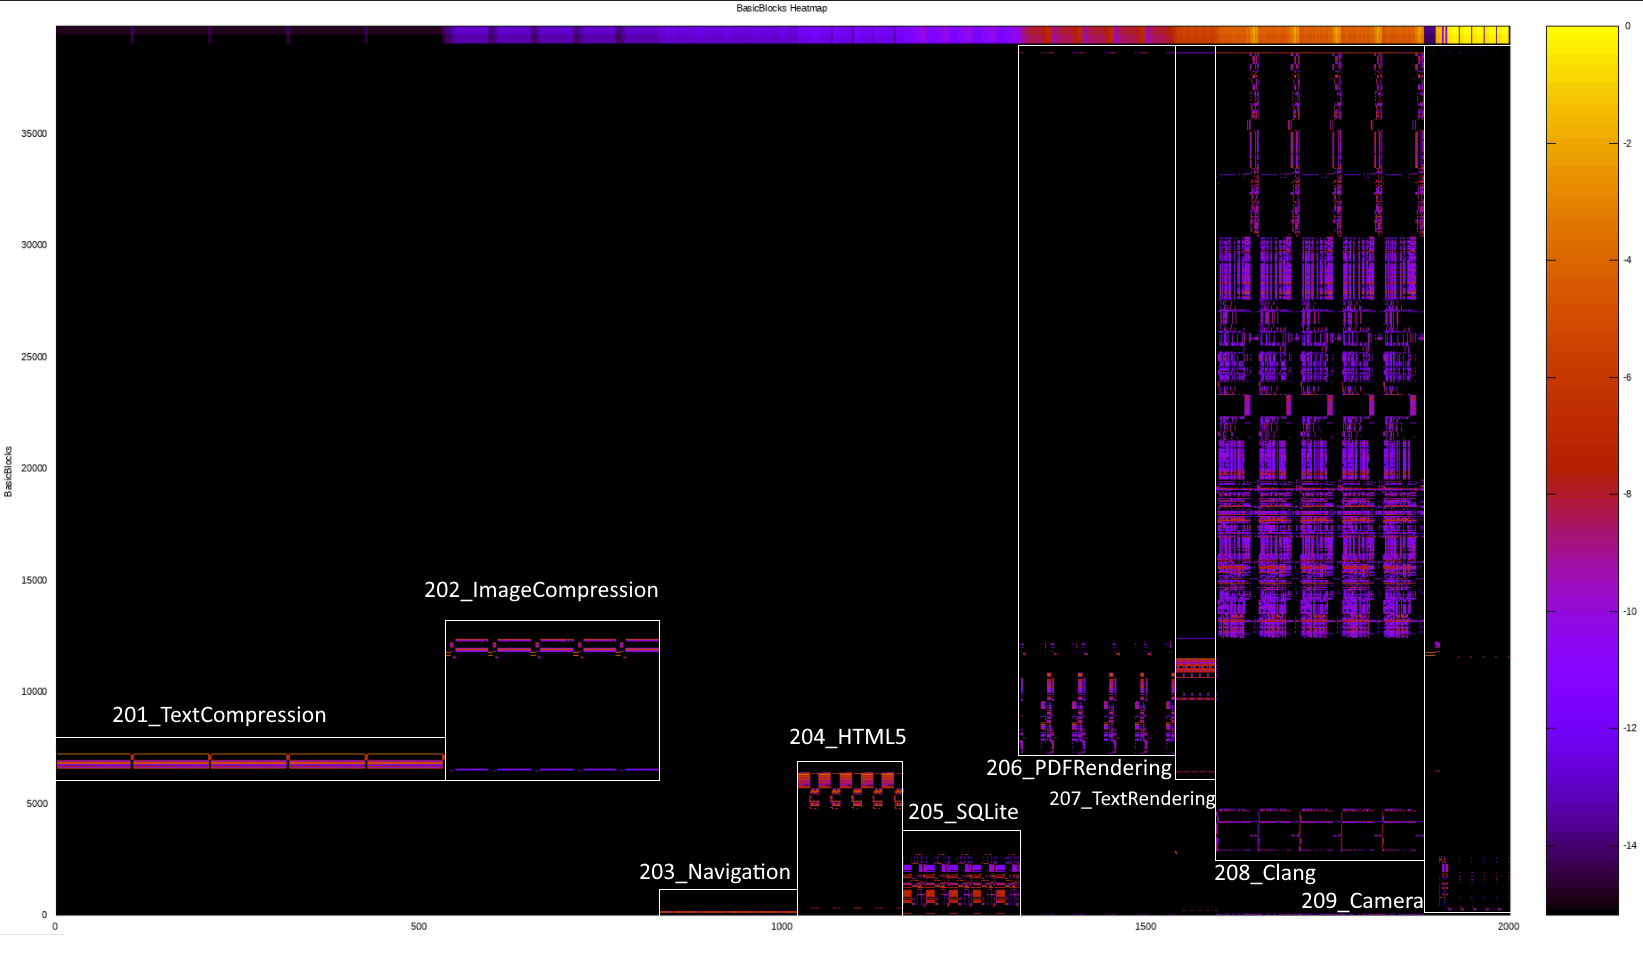
\includegraphics[width=1.0\linewidth]{_16}
    }
    \caption{Тепловая карта набора тестов Geekbench с выделенными тестами}\label{fig:GKBMP}
\end{figure}

После проведенного анализа и модификации профильной информации производится оптимизация с помощью бинарного оптимизатора BOLT (рисунок \cref{fig:CmpPerfGKB}). По результатам запуска удалось получить прирост производительности до 4\% для некоторых отдельных тестов из набора. При этом прирост на всех тестах не превышает 1\%, это связано с отсутствием больших пересечений в коде набора тестов \cite{vakbib2}.
 
\begin{figure}[!h]
    \centerfloat{
        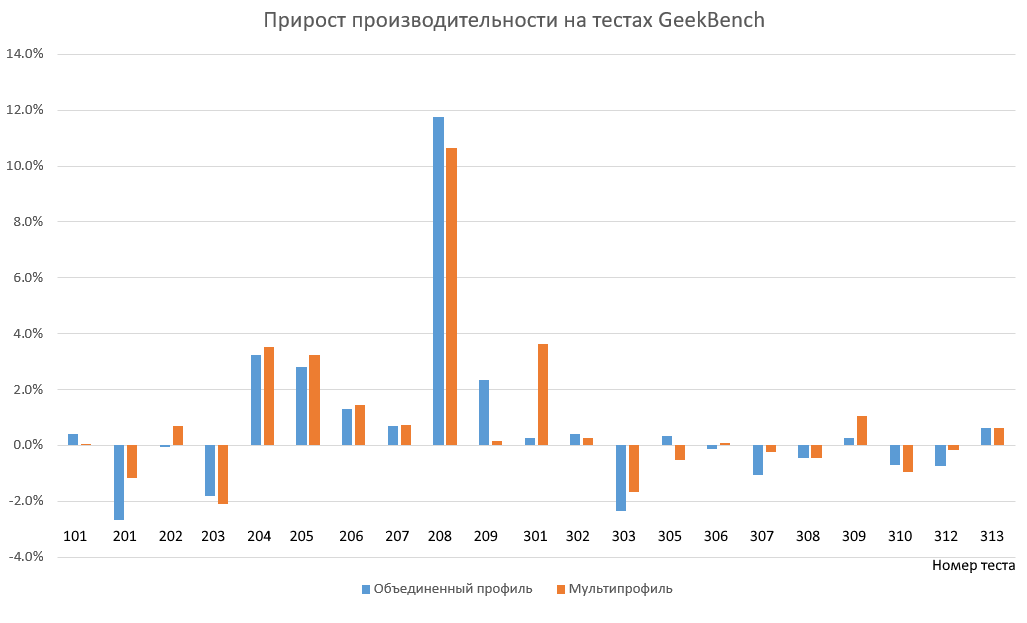
\includegraphics[width=1.0\linewidth]{_18}
    }
    \caption{Сравнение прироста производительности}\label{fig:CmpPerfGKB}
\end{figure}

При использовании оптимизации дублирования кода на основе мультипрофильной информации получаются результаты, приведенные на рисунке \cref{fig:MPResGKB}.


\begin{figure}[!h]
    \centerfloat{
        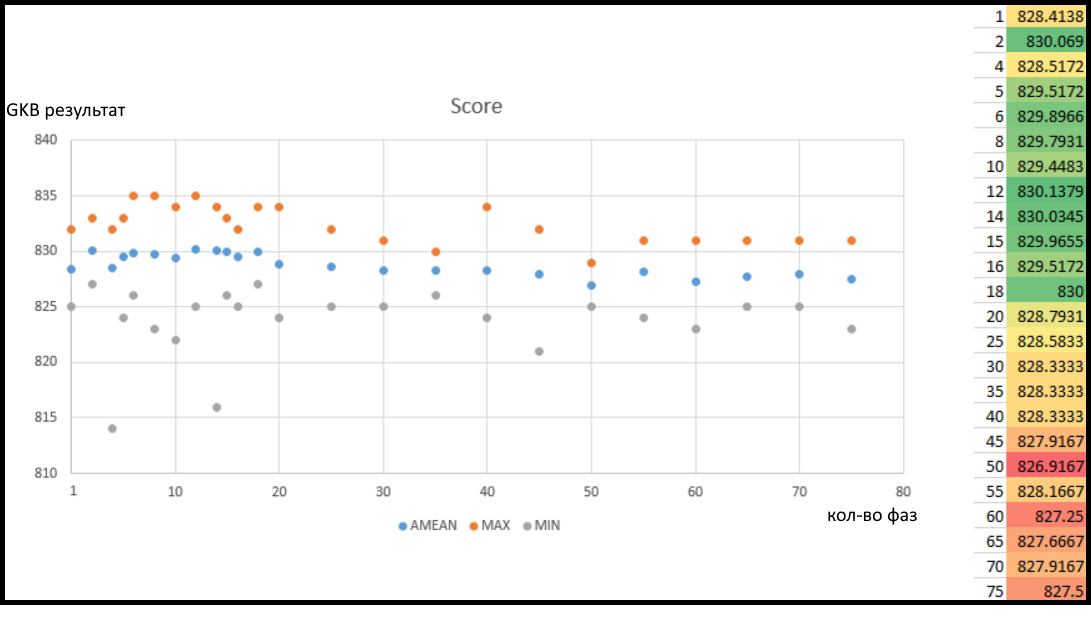
\includegraphics[width=1.0\linewidth]{scores}
    }
    \caption{Результаты тестирования мультипрофильного дублирования кода}\label{fig:MPResGKB}
\end{figure}

\section{Вывод по главе}\label{sec:ch4/sect3}
В четвертой главе были рассмотрены дополнительные оптимизации, которые можно реализовать, используя информацию из трасс исполнения. В результате проделанной работы исследованы алгоритмы мультипрофильного анализа и написан анализатор приложений на основе трасс исполнения. Разработана визуализация тепловой карты линейных участков. Анализ с оптимизацией проверены на синтетических тестах и на тестовом наборе Geekbench.


\clearpage
